\documentclass[a4paper,12pt,twoside]{article}
\usepackage[polish]{babel}
\usepackage[utf8]{inputenc}
\usepackage[T1]{fontenc}
\usepackage{graphicx}
\usepackage{anysize}
\usepackage{enumerate}
\usepackage{fancyhdr}
\usepackage{float}
\usepackage{tikz}

\begin{document}

\begin{figure}[!htb]
\centering
\begin{tikzpicture}
\draw[->] (-6.5,0) -- (6.5,0);
\draw[->] (0,-2) -- (0,2);
\node at (0,0) {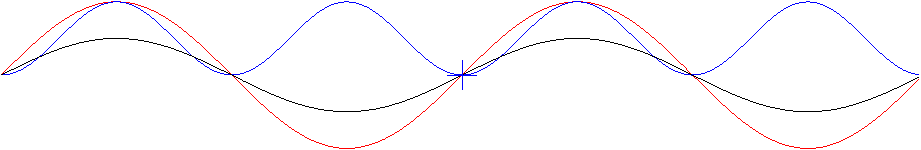
\includegraphics[scale=0.8]{f1}};
\node at (4.7,-1.2) {$f(x) = \sin(x)$};
\node at (4.7, 1.2) {$g(x) = \sin^{2}(x)$};
\node at (1.5, -0.5) {$h(x) = \frac{\sin(x)}{2}}$};
\end{tikzpicture}
\caption{Wykresy funkcji}
\label{fig:funkcje}
\end{figure}

\end{document}